% -------------------------- SETTINGS --------------------------- %
\documentclass[a4paper,11pt]{kth-mag} % Shouldn't use {openany}
\let\ifpdf\relax                    % To make the hyperref package work (MacTex doesn't like this!)
\usepackage{lmodern}                % Latin modern fonts
\usepackage[T1]{fontenc}
\usepackage[utf8]{inputenc}         % For Icelandic/Swedish characters
\usepackage{textcomp}               % Allows the use of extra characters
\usepackage[swedish,english]{babel} % For Swedish/English hyphenation patterns
\usepackage{datetime2}              % For setting the date format
\usepackage{modifications}          % KTH Template modifications
\usepackage{mathtools}              % Math support
\usepackage{amsfonts}               % This provides all the number set symbols (or \usepackage{amssymb})
\usepackage{dsfont}                 % This provides nicer font for the R symbol
\usepackage{graphicx}               % For images
\usepackage{titlesec}               % For changing chapter heading style
\usepackage{ifthen}                 % To enable if-else statements for the debug command
\usepackage[htt]{hyphenat}          % Fix hyphenation
\usepackage{hyperref}               % Adds hyper links to TOC and references (very nice). Must be the last package added apparently!
\usepackage{listings}               % For displaying code
\usepackage{enumitem}               % For styling enumerations (e.g. description environment)
\usepackage[section]{placeins}      % Testing this package for figure placement
\usepackage{pdfpages}               % For the KTH cover
\newcommand{\setdebug}{false}       % Flag for debug messages (true = display debug messages)
%!TEX root = thesis.tex

% ------------------- LAYOUT MODIFICATIONS ---------------------- %
% Equation numbers: (section_nr.equation_nr)
\numberwithin{equation}{section}

% ----------------------- CUSTOM COMMANDS ----------------------- %

% equal sign with 'def'
\newcommand{\defeq}{\ensuremath{\stackrel{\mathrm{def}}{=}}}

% The Gaussian function
\newcommand{\gaussian}[1] {\ensuremath{\frac{1}{\sqrt{2 \pi}} e^{-\frac{(#1)^2}{2}}}}
\newcommand{\gaussianexppart}[1] {\ensuremath{\exp\bigg(\frac{(#1)^2}{2}\bigg)}}
\newcommand{\gaussianexp}[1] {\ensuremath{\frac{1}{\sqrt{2 \pi}} \gaussianexppart{#1}}}

% Expectation
\newcommand{\Ex}{\mathop{\textbf E\/}}

% Command for displaying debug messages when the setdebug flag is true
\newcommand{\debug}[1]
{
  \ifthenelse{\equal{\setdebug}{true}}{DEBUG: \textbf{#1}}{}
}

% Argmax and argmin
\newcommand{\argmax}[1]{\underset{#1}{\operatorname{arg}\,\operatorname{max}}\;}
\newcommand{\argmin}[1]{\underset{#1}{\operatorname{arg}\,\operatorname{min}}\;}

% Big-O
\newcommand{\BigO}[1]{\ensuremath{\operatorname{O}\bigl(#1\bigr)}}

\DTMsetstyle{iso}                   % Swedish date format on flyleaf page

% --------------------------- THESIS ---------------------------- %
\title{Partially Observable Markov Decision Processes for Faster Object Recognition}

\author{Björgvin Olafsson}
\email{bjoola@kth.se}

\blurb{DD221X, Master’s Thesis in Computer Science (30 ECTS credits)
\\Master’s Programme in Machine Learning 120 credits
\\Supervisor at KTH: Andrzej Pronobis
\\Supervisor at principal: Babak Rasolzadeh
\\Examiner: Stefan Carlsson
\\Principal: OculusAI Technologies AB}
\date{\today}
\trita{}

\begin{document}

\frontmatter
\pagestyle{empty}
\removepagenumbers
\includepdf[pages={1}, pagecommand={}]{kth-cover.pdf}
\maketitle

%!TEX root = thesis.tex

\selectlanguage{english}
\begin{abstract}

Object recognition in the real world is a big challenge in the field of computer vision. Given the potentially enormous size of the search space it is essential to be able to make intelligent decisions about where in the visual field to obtain information from to reduce the computational resources needed.

In this report a POMDP (Partially Observable Markov Decision Process) learning framework, using a policy gradient method and information rewards as a training signal, has been implemented and used to train fixation policies that aim to maximize the information gathered in each fixation. The purpose of such policies is to make object recognition faster by reducing the number of fixations needed. The trained policies are evaluated by simulation and comparing them with several fixed policies. Finally it is shown that it is possible to use the framework to train policies that outperform the fixed policies for certain observation models.

\end{abstract}
\clearpage

%!TEX root = thesis.tex

\clearpage
\thispagestyle{empty}
\chapter*{Acknowledgments}

I would like to express my deepest appreciation to all those who provided me the possibility to complete this project.
\\
\\
Special thanks to my supervisor for his infinite wisdom and knowledge and all the support throughout the course of this project. I would also like to thank the whole team at OculusAI for a fantastic journey.
\\
\\
Furthermore, I would like to thank Andreas and Siamak for getting me motivated to finish the work I started.
\\
\\
And finally, I would like to thank my parents for always being there for me and my partner Moa for her support and incredible patience.
\clearpage


\tableofcontents*

% ------------------------ MAIN MATTER -------------------------- %
\mainmatter

%!TEX root = thesis.tex

\pagestyle{newchap}

\chapter{Introduction}
One of the biggest challenges in the field of computer vision today is object recognition in the real world. The amount of information available to be perceived at any given point in the world is enormous so making intelligent decisions about where to obtain information from is essential for literally any task. This is important for us humans in our daily lives and even more important for machines that are set out to solve difficult tasks in the real world.

Humans use eye movements to focus on specific areas in the visual field and visual attention is the mechanism that decides which area to focus on, i.e. where to obtain information from, which greatly reduces the search space. When it comes to machines this problem is typically solved using the \emph{sliding window} approach, where a window of a specific size is slided over an image and in each position only the part of the image that is visible through the window is processed. The window size and the amount of overlap between positions can be varied. Visual attention can be simulated with this approach by using fast and simple detectors to quickly identify areas in an image that are of little interest and applying more accurate detectors on other areas of the image.

In order to make intelligent decisions, one needs to make use of information and the quality of that information is a key factor for the quality of the decision making itself. In general, searching for an object in an image requires every part of the image to be processed, one by one, until either the object is found or all parts have been processed with negative results. Being able to derive a strategy that determines which parts of an image should be processed first, based on the expected information to be gained from processing each part, could potentially result in a faster and more intelligent way of searching for objects in images.

This report was written for OCULUSai Technologies AB, a Swedish computer vision company that focuses on product recognition. One of the main problems the company is trying to solve is recognition of shoes, bags and other fashion items in photos taken by consumers on their mobile devices. One step in that process is to detect if the item in question is present in a photo and where it is located.

In this report a learning framework, using a method for learning information\hyp{}gathering strategies \cite{Butko2010b}, has been implemented and evaluated by simulation, and an example of how the framework might be used to enhance performance of an object detection algorithm is discussed.

\section{Contributions}

The goal of this thesis is to implement a POMDP (Partially Observable Markov Decision Process) learning framework that uses a policy gradient method and information rewards as a training signal for learning policies that maximize information. The learning framework will be evaluated by simulation and comparing the learned policies with fixed policies, and its potential use in object detection in images will be discussed.

\section{Related Work}
Information\hyp{}gathering strategies have been successfully used to learn optimal policies for control of eye movements \cite{Butko2010b}, for speeding up reinforcement learning in POMDPs \cite{Fasel2011a} and for acoustic exploration of objects \cite{Fasel2011b} to name a few examples.
Employing a selective information\hyp{}gathering strategy in a mobile robot, where the robot reasons whether deviating from the shortest path to a goal in order to get to a more suitable vantage point is beneficial or not, has been shown to improve the precision of object detections \cite{Velez2011}.
The policy gradient method used in this report is presented in \cite{BaxterB2001}.

\section{Outline}
Chapter \ref{ch:Background} introduces the fundamentals of the POMDP framework and its extensions towards information-driven policies. Chapter \ref{ch:IPOMDP} describes the scenario used for evaluation and presents problem specific models. Chapter \ref{ch:Implementation} presents the POMDP learning framework that was implemented and provides information on how it can be used. In Chapter \ref{ch:Evaluation} the implementation is evaluated by training information\hyp{}gathering policies and comparing them with several fixed policies. Finally, in Chapter \ref{ch:Conclusions}, the conclusions and future work are discussed along with the potential use of the framework for object detection.

Appendix \ref{app:Derivations} contains derivations and equations used in the report and Appendix \ref{app:GradientCImplementation} contains a C implementation of the policy gradient method, described in Section \ref{sec:PolicyGradient}.

%!TEX root = thesis.tex

\chapter{Background}
\label{ch:Background}
This chapter introduces the theory behind the implemented method and the terminology used in this report.

The notation used in the report is as follows. Upper-case letters are used for random variables, e.g. $O_t$ for the random variable of observations at time $t$. Lower-case letters are used to indicate specific values of the corresponding random variable, e.g. $o_t$ represents a specific value of the random variable $O_t$.

\section{Formulation and Terminology of POMDPs}
A Markov decision process (MDP) is a mathematical framework for modeling sequential decision making problems and the framework forms the basis for the POMDP framework, which is a generalization of MDPs. In the MDP framework the state of the world is directly observable whereas in the POMDP framework it is only partially observable. When the state of the world cannot be determined directly a probability distribution over all the possible states of the world must be maintained. More detailed information about POMDPs can be found in \cite{Kaelbling1998} and \cite{Aberdeen2003}.

\subsection{The POMDP World Model}
\label{sec:POMDPModel}
The acting entity in the POMDP world model, the learner, is called an \emph{agent}. The world model in the POMDP framework consists of the following:

\begin{itemize}
  \item $\mathcal{S} = \{1, \dotsc, |\mathcal{S}|\}$ -- States of the world.
  \item $\mathcal{A} = \{1, \dotsc, |\mathcal{A}|\}$ -- Actions available to the agent.
  \item $\mathcal{O} = \{1, \dotsc, |\mathcal{O}|\}$ -- Observations the agent can make.
  \item Reward $r(i) \in \mathds{R}$ for each state $i \in \mathcal{S}$.
\end{itemize}
At time $t$, in state $S_t$, the agent takes an action $A_t$ according to its policy, makes an observation $O_t$, transitions to a new state $S_{t+1}$ and collects a reward $r(S_{t+1})$ according to the reward function $r(i)$. The state transition is made according to the system dynamics that are modeled by the transition model discussed in \ref{sec:TransitionModel}. Figure \ref{fig:POMDPModel} illustrates this along with the relations between MDPs and POMDPs.

\begin{figure}[ht]
  \centering
  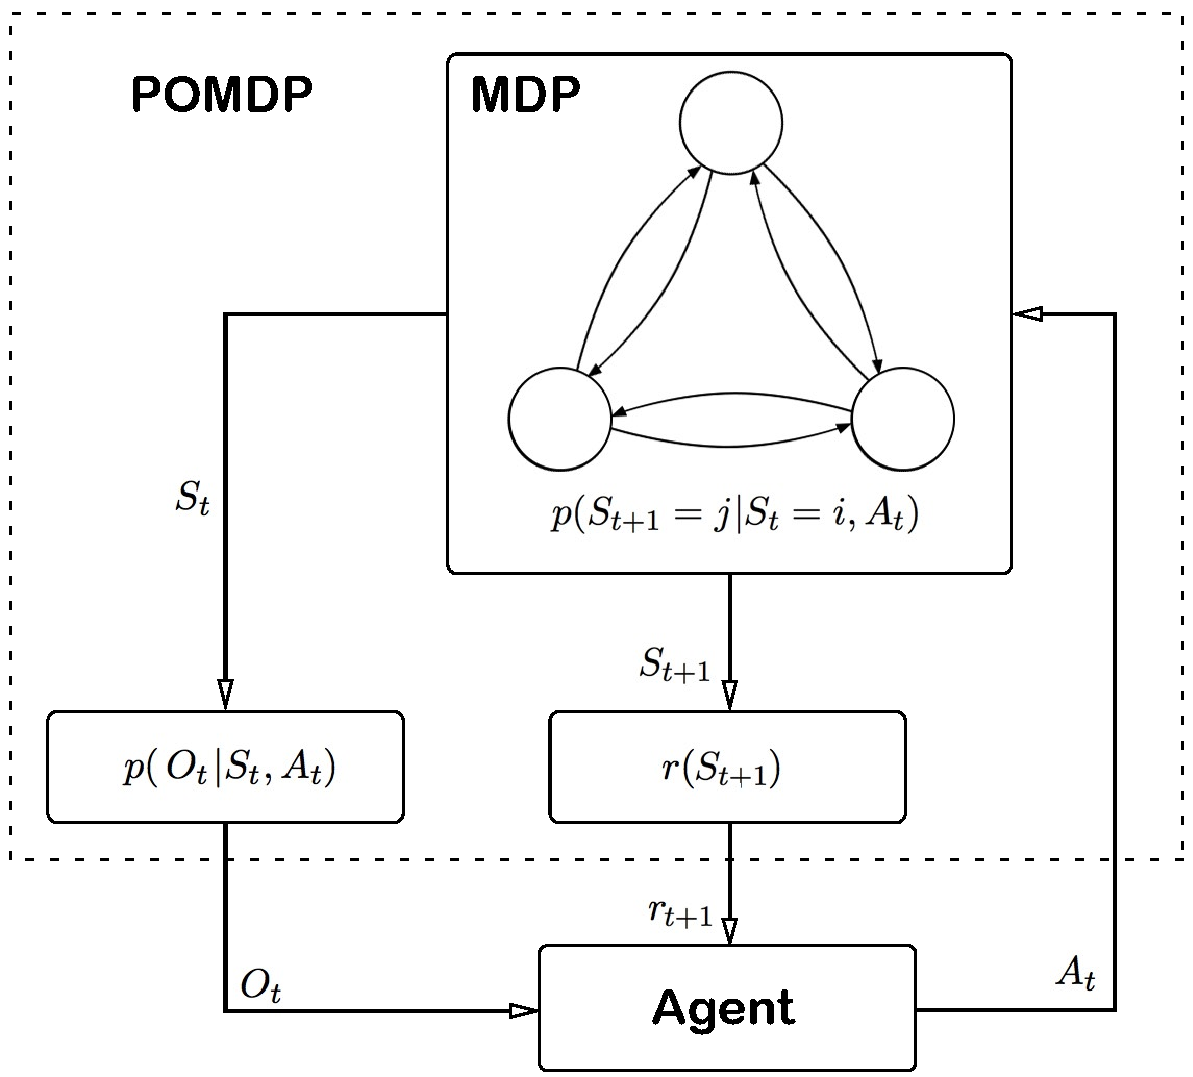
\includegraphics[width=0.5\textwidth]{figures/pomdp_model}
  \caption{POMDP diagram. In an MDP the agent would observe the state, $S_t$, directly. In POMDPs the agent makes an observation, $O_t$, that is mapped to the state $S_t$ by a stochastic process. Figure adapted from \cite{Aberdeen2003}.}
  \label{fig:POMDPModel}
\end{figure}

To put these concepts into context consider the problem of a robot that needs to find its way out of a maze. In the POMDP world model for that problem the robot is the agent and the state could be the location of the robot in the maze. The actions could be that the robot decides to move in a certain direction or even use one of its sensors. An observation could then be a reading from that sensor.

Since this example is easy to grasp it will be used throughout this report where deemed necessary.

\subsection{Transition Model}
\label{sec:TransitionModel}
The transition model defines the probabilities of moving from the current state to any other state of the world for any given action. For each state and action pair $(S_t = i, A_t = k)$ we write the probability of moving from state $i$ to state $j$ when action $A_t = k$ is taken as
\begin{equation}
  p(S_{t+1} = j|S_t = i, A_t = k)
\end{equation}
When a transition from state $i$ to state $j$ is for some reason impossible given action $k$, this probability is zero. An example of this would be when the agent takes an action that is intended to sense the environment and not move the agent. When the system dynamics prohibit all transitions, i.e. the state never changes, this probability is 1 for $i = j$ and zero otherwise, i.e.
\begin{equation}
\label{eq:IdentityTransitionModel}
  p(S_{t+1} = j|S_t = i, A_t = k) = 
  \begin{cases}
    1 & \text{if $i = j$}\\
    0 & \text{otherwise}
  \end{cases}
\end{equation}
The transition model for a specific problem is generally known or estimated using either empirical data or simply intuition.

\subsection{Belief States}
Because of the partial observability the agent is unable to determine its current state. However, the observations the agent makes depend on the underlying state so the agent can use the observations to estimate the current state. This estimation is called the agent's belief, or the belief state.
\begin{equation*}
  \mathcal{B} = \{1, \dotsc, |\mathcal{B}|\} \text{ -- Belief states, the agent's belief of the state of the world.}
\end{equation*}
A single belief state at time $t$, $B_t$, is a probability distribution over all states $i \in \mathcal{S}$. The probability of the state at time $t$ being equal to $i$, given all actions that have been taken and observations that have been made, is defined as
\begin{equation}
  B_t^i \defeq p(S_t = i | A_{1:t}, O_{1:t})
\end{equation}
Each time the agent takes an action and makes a new observation it gains more information about the state of the world. The most obvious way to keep track of this information is to store all actions and observations the agent makes, but that results in an unnecessary use of memory and computing power. It is possible to store all the acquired information within the belief state and update it only when necessary, after taking actions and making observations, without storing the whole history of actions and observations.

Given the belief state $b_t$, current action $a_t$ and observation $o_t$ the belief for state $j$ can be updated using
\begin{equation}
  \label{eq:UpdateBelief}
  b_t^j = \frac{ p(o_t | S_t = j, a_t) \sum_{i} p(S_t = j | S_{t-1} = i, a_t) b_{t-1}^i } { p(o_t) }
\end{equation}
If the state never changes we can simplify equation \eqref{eq:UpdateBelief} to

\begin{equation}
  \label{eq:UpdateBeliefFixedTarget}
  b_t^j = \frac{ p(o_t | S_t = j, a_t) b_{t-1}^j }{ p(o_t) }
\end{equation}
where $p(o_t)$ can be treated as a normalization factor. The derivations of \eqref{eq:UpdateBelief} and \eqref{eq:UpdateBeliefFixedTarget} are presented in Appendix \ref{app:BeliefUpdates}.

\subsection{Reward Function}
\label{sec:RewardFunction}
After each state transition the agent gets a reward according to the reward function. These rewards are the agent's indication of its performance and they are generally extrinsic and task-specific. In the case of a robot finding its way out of a maze the reward function might return a small negative reward for all states the robot visits and a large positive reward for the end state, i.e. when the robot is out of the maze, as described in \ref{sec:ModelBasedvsModelFree}. Since the goal is to find a policy that maximizes the expected total rewards the robot will learn to find the shortest path out of the maze.

The reward function may depend on the current action and either the current or the resulting state, but it can be made dependent on the resulting state only without loss of generality \cite{Aberdeen2003}. In Section \ref{sec:InformationRewards} we show how a reward function can be made dependent on the belief state only.

\subsection{Policy}
When it is time for the agent to act it consults its policy. The agent's policy is a mapping from states to actions that defines the agent's behavior. Finding a solution to a POMDP problem is done by finding the optimal policy, i.e. a policy that provides the optimal action for every state the agent visits, or approximating it when finding an exact solution is infeasible.

We already know that in POMDPs the agent is unable to determine its current state and a mapping from states to actions is therefore useless for the agent. The straightforward solution to this is to make the policy depend on the belief state. That is typically done by parameterizing the policy as a function of the belief state. Finding or approximating the optimal policy therefore becomes a search for the optimal policy parameters. 

\subsection{Logistic Policies}
\label{sec:LogisticPolicies}
One way of parameterizing a policy is to represent it as a function with policy parameters $\theta \in \mathds{R^{|\mathcal{A}| \times |\mathcal{S}|}}$, where $\mathcal{A}$ is the set of actions available to the agent and $\mathcal{S}$ the set of states of the world as presented in \ref{sec:POMDPModel}. Then $\theta$ forms a $|\mathcal{A}| \times |\mathcal{S}|$ matrix which in combination with the current belief state, $b_t$, forms a set of linear functions of the belief state. If $\theta^i$ represents the $i$th row of the matrix $\theta$ then we can select an action according to the policy with
\begin{equation}
  a_{t+1} = \argmax{i} \theta^i \cdot b_t
\end{equation}
This is a deterministic policy since it will always result in the same action for a particular belief state $b_t$. However, if we need a stochastic policy -- as is the case for the policy gradient method described in \ref{sec:GradientAscent} -- we can represent it as a logistic function using the policy parameters $\theta$ and the current belief state, $b_t$. Again, if $\theta^i$ represents the $i$th row of the matrix $\theta$ then the probability of taking action $k$ is given by
\begin{equation}
\label{eq:LogisticPolicy}
  p(A_{t+1} = k | b_t, \theta) = \frac{ \exp{(\theta^k \cdot b_t)} }{ \sum_{i=1}^{|\mathcal{A}|}{ \exp{( \theta^i \cdot b_t}) }} 
\end{equation} 
where $b_t$ is the agent's belief. This is a probability distribution that represents a stochastic policy. Taking an action based on this stochastic policy is done by sampling from the probability distribution.

The key to estimating the policy gradient in equation \eqref{eq:PolicyGradient} lies in calculating the gradient of equation \eqref{eq:LogisticPolicy} with respect to $\theta$, as shown in \cite{Butko2010b}.

\subsection{Observation Model}
\label{sec:ObservationModel}
When training a policy, the agent must be able to make observations. The sensors the agent uses to observe the world are in general imperfect and noisy which means that when the agent makes an observation it has to assume some uncertainty.

The observations available to the agent can be actual readings from its sensors -- and that is the case when the agent is put to work in the real world -- but during training, having a model that can generate observations is preferred. This is called an observation model and its purpose is to model the noisy behavior of the actual sensors.

The observation model needs to be estimated or trained using real data acquired by the agent's sensors before training the policy.

\subsection{Observation Likelihood}
\label{sec:ObservationLikelihood}
The observation likelihood is the probability of making observation $O_t$ after the agent takes action $A_t$ in state $S_{t}$,
\begin{equation}
  p(O_t|S_t, A_t)
\end{equation}
given the current observation model.

\subsection{Model-based vs. Model-free}
\label{sec:ModelBasedvsModelFree}
When the observation model, the transition model and the reward function $r(i)$ are all known, the POMDP is considered to be \emph{model-based}. Otherwise the POMDP is said to be \emph{model-free}.

A model-free POMDP can learn a policy without a full model of the world by sampling trajectories through the state space, either by interacting with the world or using a simulator. To give an example, consider our robot friend again that needs to find its way out of a maze. If the robot receives a small negative reward in each state it visits and a large positive reward when it gets out, it can learn a policy by exploring the maze without necessarily knowing the transition model or observation model.

The POMDPs considered in this report are always model-based.

\section{Policy Gradient}
\label{sec:PolicyGradient}
Methods for finding exact optimal solutions to POMDPs exist but they become infeasible for problems with large state- and action-spaces and they require full knowledge of the system dynamics, such as the transition model and the reward function. When either of those requirements are not fulfilled, reinforcement learning can be used to estimate the optimal policy.

The methods used, when exact methods are infeasible, are either value function methods or direct policy search. Value function methods require the agent to assign a value to each state and action pair and this value represents the long term expected reward for taking an action in a given state. In every state the agent chooses the action that has the highest value given the state, so the policy is essentially extracted from the value function. As the state-space grows larger the value function becomes more complex, making it more challenging to learn. However, the policy-space does not necessarily become more complex, making it more desirable to search the policy-space directly \cite{Aberdeen2003}. 

An algorithm for a direct policy search using gradient ascent was presented in \cite{BaxterB2001} and used in \cite{Butko2010b}. The algorithm generates an estimate of the gradient of the average reward with respect to the policy and using gradient ascent the policy is improved iteratively. This requires a parameterized representation of the policy.

\subsection{Gradient Ascent}
\label{sec:GradientAscent}
If the policy is parameterized by $\theta$, for example as described in \ref{sec:LogisticPolicies}, the average reward of the policy can be written as 
\begin{equation}
  \underbrace{\eta(\theta)}_{\mathclap{\substack{\text{Average} \\ \text{reward}}}} = \sum_{x \in X} \underbrace{r(x)}_{\text{reward}} \overbrace{p(x | \theta)}^{\substack{\text{prob. of $x$} \\ \text{given policy}}} = \Ex [r(x)]
\end{equation}
where $x$ represents the parameters that the reward function depends on. In our case $x$ is the agent's belief, $b$. The gradient of the average reward given the parameterized policy $\theta$ is therefore
\begin{align}
  \nabla \eta(\theta) &= \sum_{b \in \mathcal{B}} r(b) \nabla p(b | \theta) \\
                      &= \sum_{b \in \mathcal{B}} r(b) \frac{\nabla p(b | \theta)}{p(b | \theta)} p(b | \theta) \\
                      &= \Ex \bigg{[}r(b) \frac{\nabla p(b | \theta)}{p(b | \theta)}\bigg{]}
\end{align}
If we generate $N$ i.i.d. samples from $p(b | \theta)$ then we can estimate $\nabla \eta(\theta)$ by
\begin{equation}
  \widetilde{\nabla} \eta(\theta) = \frac{1}{N} \sum_{i=1}^N r(b_i) \frac{\nabla p(b_i | \theta)}{p(b_i | \theta)}
  \Bigg{\}} \substack{\text{given fixed $\theta$} \\ \text{we sample $b_i$} \\ \text{and we estimate} \\ \text{$\nabla \eta(\theta)$}}
\end{equation}
with $N \to \infty$, $\widetilde{\nabla} \eta(\theta) \to \nabla \eta(\theta)$.
\\\\
Assume a regenerative process, each i.i.d. $b_i$ is now a sequence $b_i^1 \dotsc b_i^{M_i}$.
We get
\begin{equation}
  \widetilde{\nabla} \eta(\theta) = \frac{1}{N} \sum_{i=1}^N r(b_i^1, \dotsc, b_i^{M_i}) \sum_{j=1}^{M_i} \frac{\nabla p(b_i^j | \theta)}{p(b_i^j | \theta)}
\end{equation}
If we assume
\begin{equation}
  r(b_i^1, \dotsc, b_i^{M_i}) = f\Big{(} \underbrace{r(b_i^1, \dotsc, b_i^{M_{i-1}})}_{r_i^{M_{i-1}}}, b_i^{M_i}\Big{)}
\end{equation}
and write
\begin{equation}
  \sum_{j=1}^{M_i} \frac{\nabla p(b_i^j | \theta)}{p(b_i^j | \theta)} = Z_i^{M_i} = Z_i^{M_{i-1}}  + \frac{\nabla p(b_i^{M_i} | \theta)}{p(b_i^{M_i} | \theta)}
\end{equation}
we have
\begin{equation}
  \widetilde{\nabla} \eta(\theta) = \frac{1}{N} \sum_{i=1}^N \underbrace{r_i^{M_i} Z_i^{M_i}}_{\substack{\text{Computed} \\ \text{iteratively}}} \bigg{\}} \frac{1}{N} \widetilde{\nabla}_N
\end{equation}
where
\begin{equation}
  r_i^{M_{i}} = r(b_i^1, \dotsc, b_i^{M_i})
\end{equation}
This gives an unbiased estimate of the policy gradient
\begin{equation}
  \label{eq:GradientEstimate}
  \underbrace{\widetilde{\nabla}_N}_{\substack{\text{Computed} \\ \text{iteratively}}} = \widetilde{\nabla}_{N-1} + r_N^{M_N} Z_N^{M_N}
\end{equation}
The estimate of the gradient of the average reward, $\widetilde{\nabla}_N$, can therefore be computed iteratively and the policy parameters $\theta$ updated by a simple update rule 
\begin{equation}
\label{eq:PolicyGradient}
  \theta_{new} = \theta + \frac{\widetilde{\nabla}_N}{N}
\end{equation}
where $N$ is the number of samples used to estimate the gradient, i.e. the number of episodes.

When training a policy using gradient ascent the gradient of the average reward is estimated from a number of episodes, during which the policy parameters are kept fixed. When all episodes have finished the policy parameters are updated using the gradient estimation and that concludes one training iteration, a so called epoch.

The gradient estimate is what has been referred to as the policy gradient.

\section{Infomax Control}
Using the theory of optimal control in combination with information maximization is known as \emph{Infomax control} \cite{Movellan2005}. The idea is to treat the task of learning as a control problem where the goal is to derive a policy that seeks to maximize information, or equivalently, reduce the total uncertainty. The POMDP models that are used for this purpose are information gathering POMDPs and have been called Infomax POMDPs, or I-POMDPs \cite{Butko2010b}.

\section{Information Rewards}
\label{sec:InformationRewards}
Conceptually, the POMDP world issues rewards to the agent as it interacts with the world and these rewards are generally task-specific. In order to make an information-driven POMDP, an I-POMDP, the reward function must depend on the amount of information the agent gathers. The way this is done is to make the reward a function of the agent's belief of the world. The entropy of the agent's belief at each point in time becomes the reward the agent receives. As the agent becomes more and more certain about the state of the world, the higher reward the agent receives. This principle is what drives the learning of information gathering strategies. The policy gradient is used to adjust the current policy and the reward, i.e. the certainty of the agent's belief, controls the magnitude of the adjustment. This is shown in equation \eqref{eq:GradientEstimate}.

The information reward function becomes
\begin{equation}
\label{eq:InformationRewards}
  r_t(b_t) = \sum_{j=1}^{|\mathcal{S}|} b_t^j \log_2{b_t^j}
\end{equation}
where $\mathcal{S}$ is the set of states of the world and $b_t$ is the agent's belief at time $t$.

Care needs to be taken when calculating the logarithm of the belief in practice because as the agent becomes more certain about the state of the world, most of the values of the belief vector $b_t$ approach zero. As the precision of numbers stored in computers varies, we might have the situation where some of those values are actually stored as zero. Therefore, when calculating the rewards we define

\begin{equation}
  \log_2{0} \defeq 0
\end{equation}

%!TEX root = thesis.tex

\chapter{I-POMDPs for Object Detection}
\label{ch:IPOMDP}
The problem of object detection can be formulated as an I-POMDP using the game ``Where's Waldo?'' as an example. This example is presented in \cite{Butko2010b}. The goal of the game is to find a person, Waldo, in an illustrated image full of people and objects that have similar appearance as Waldo himself. For the evaluation we assume we have a detector that recognizes Waldo but the people and objects that are similar to Waldo act as noise in the detector.

From the agent's point of view, the goal in the ``Where's Waldo?'' game is to find Waldo in an image by fixating on different parts of the image using as few fixations as possible. To accomplish that the agent needs to learn a good policy. The policy determines which part of the image the agent fixates on in every time step and the number of fixations needed to find Waldo gives a measure of how well the policy performs. The part of the image that Waldo occupies is the state of the world and we assume that Waldo doesn't move so the state never changes. The agent's belief for each state is  the probability of Waldo being in that state, i.e. positioned in that part of the image, given previous observations and actions.

In this chapter we describe the problem specific models that were implemented and used for evaluation of the ``Where's Waldo?'' problem.

\section{Observation Model}
\label{sec:ObservationModelImpl}
Two different observation models are used for the evaluation. The first one is a model where the agent's ability to distinguish between a signal from an object and noise decays exponentially from the point where the agent is focusing. This observation model is
\begin{equation}\label{eq:ObservationModel}
  \begin{split}
    O_t^j &= \delta (S_t, j) d_{j,k} + Z_t^j \\
          &= \begin{cases}
                d_{j,k} + Z_t^j & \text{if $S_t = j$}\\
                Z_t^j           & \text{otherwise}
             \end{cases}
  \end{split}
\end{equation}
where $Z_t^j$ is zero mean, unit variance Gaussian random noise (i.e. white noise) and
\begin{equation}
  d_{j,k} = 3 \cdot e^{-dist(j,k)}
\end{equation}
where $dist(j,k)$ is the Euclidean distance between locations $j$ and $k$.

We will call this model the \emph{Exponential model}. An example of how this vision system sees an image (without noise) can be seen in Figure \ref{fig:ObsmodelExp}.

\begin{figure}[!htp]
  \centering
  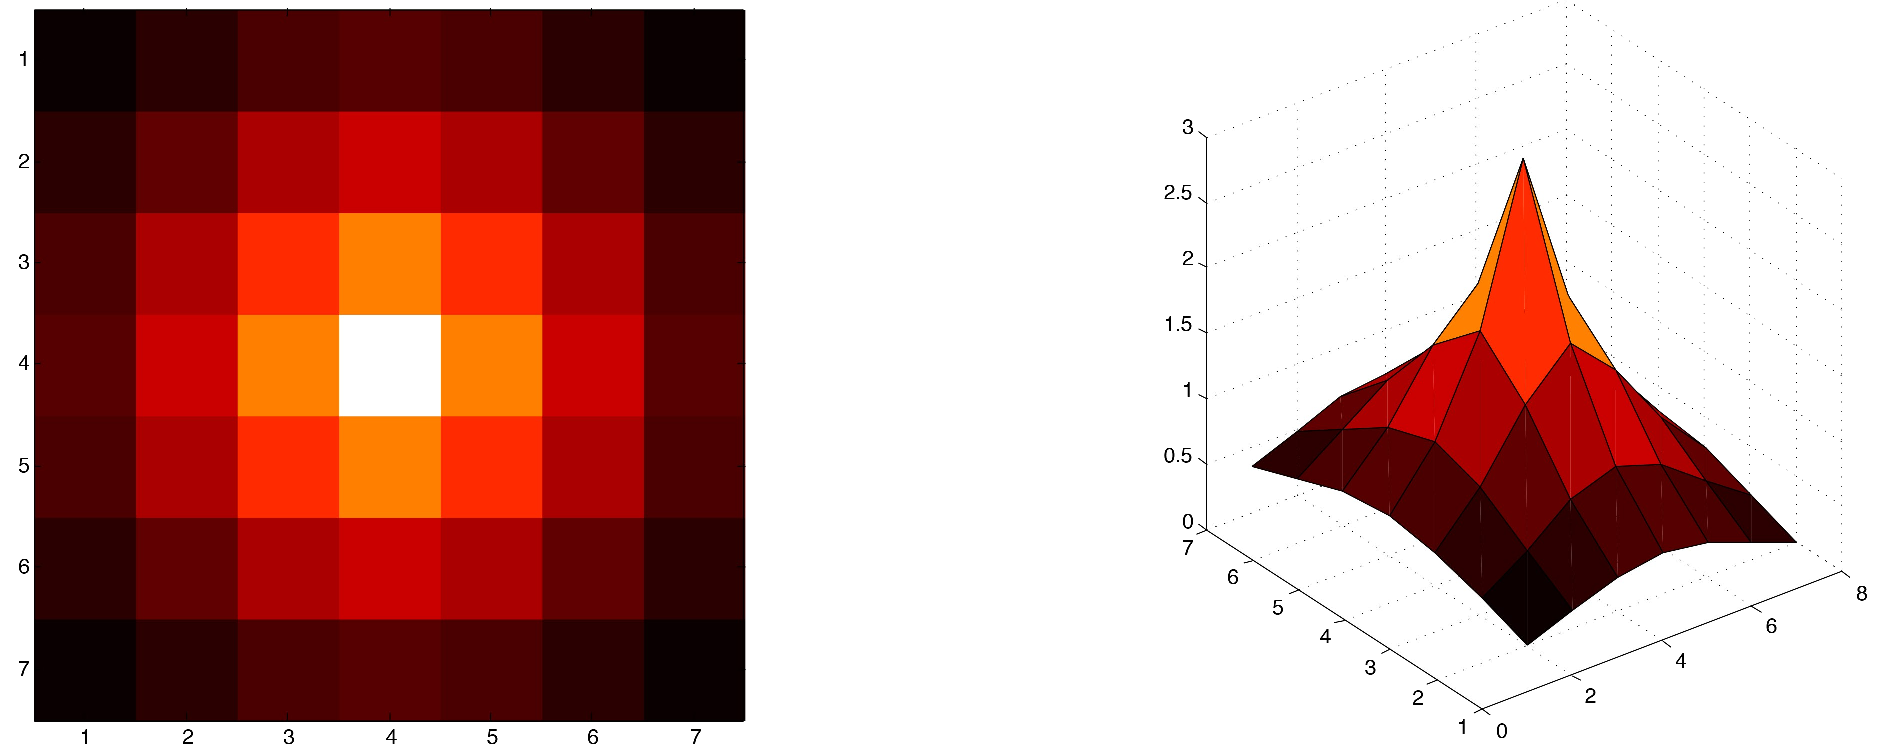
\includegraphics[width=1\textwidth]{figures/obsmodel_exp}
  \caption{A vision system with an exponential decay of focus. The agent focuses on the center of the image and the the focus point is the most reliable one. The ability to distinguish between noise and a signal from an object decreases with the distance from the agent's focus point.}
  \label{fig:ObsmodelExp}
\end{figure}

The second model is a model of the properties of the human eye. This model takes the same form as the exponential model in equation \eqref{eq:ObservationModel} but now $d_{j,k}$ is as described in \cite{Najemnik2005}.

We will call this model the \emph{Human eye model}. An example of how this vision system sees an image (without noise) can be seen in Figure \ref{fig:ObsmodelCont}.

\begin{figure}[!htp]
  \centering
  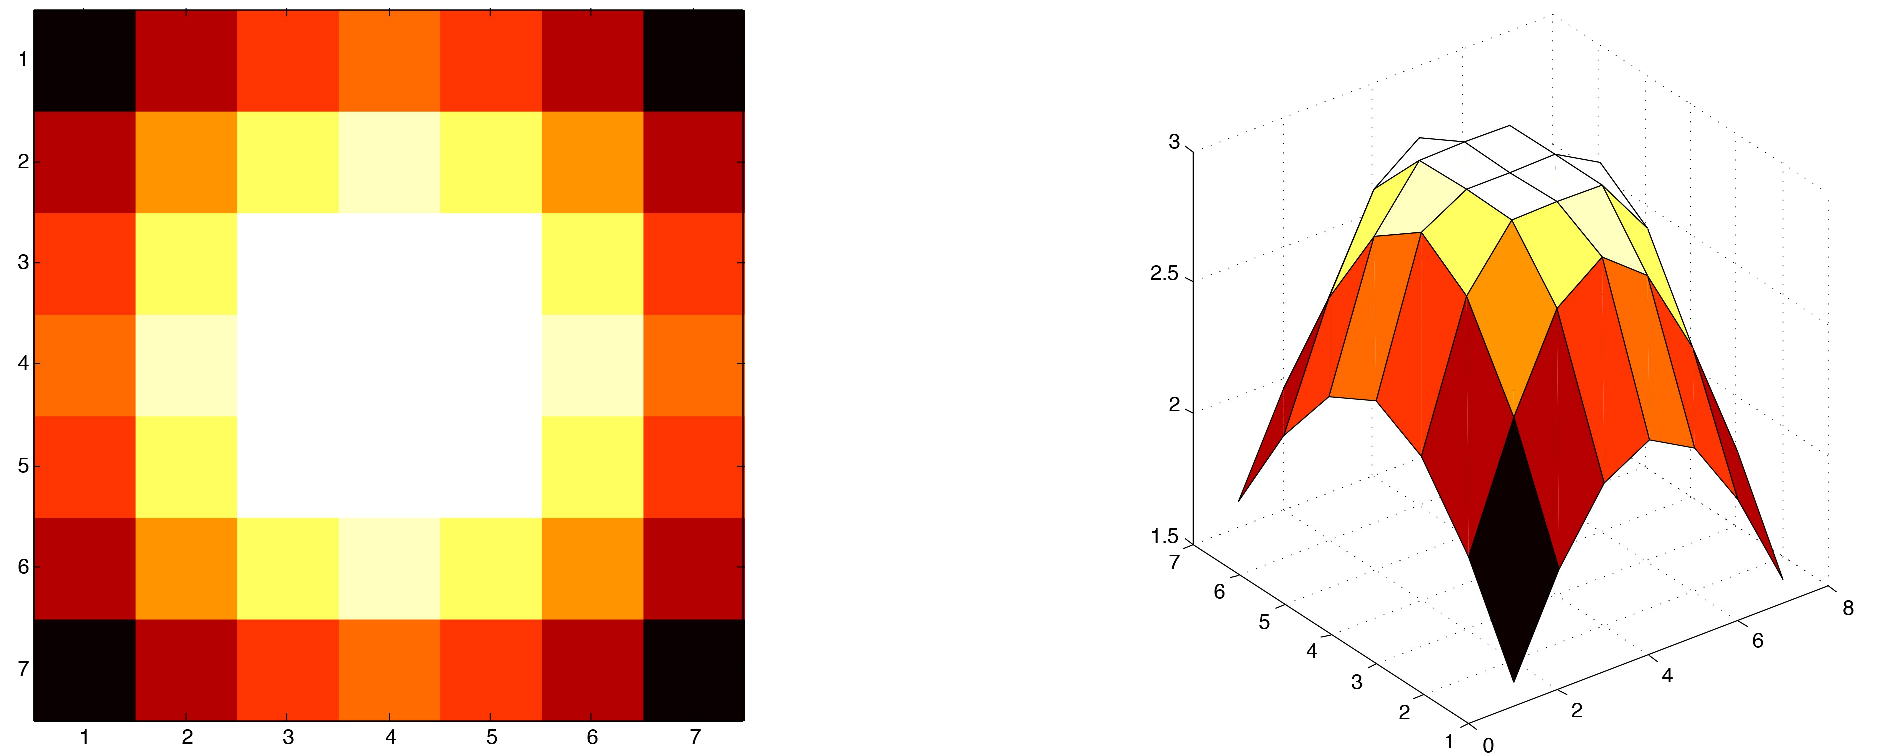
\includegraphics[width=1\textwidth]{figures/obsmodel_cont}
  \caption{A vision system with the characteristics modeled after the human eye. The agent focuses on the center of the image and is able to distinguish between noise and a signal from an object in and around the center. The reliability of the vision drops dramatically in locations further away from the agent's focus point.}
  \label{fig:ObsmodelCont}
\end{figure}

\section{Observation Likelihood}
\label{sec:ObservationLikelihoodImpl}
We assume that given an image, individual observations (i.e. each pixel or cell)
\begin{equation}
  o_t = (o_t^1, \dotsc, o_t^{|\mathcal{S}|})
\end{equation}
are conditionally independent. Then we can write the probability of an observation as
\begin{subequations}
  \begin{align}
    p(o_t | S_t = i, A_t = k) 
      &= \prod_j p(o_t^j | S_t = i, A_t = k) \\
      &= p(o_t^i | S_t = i, A_t = k) \prod_{j \neq i} p(o_t^j | S_t = i, A_t = k) \\
      \intertext{Given the observation model from equation \eqref{eq:ObservationModel} we get}
      &= \gaussianexp{o_t^i - d_{i,k}} \prod_{j \neq i} \gaussianexp{o_t^j} \\
      &= \frac{1}{\sqrt{2\pi}} \frac{\gaussianexppart{o_t^i - d_{i,k}}}{\gaussianexppart{o_t^i}} \prod_j \gaussianexp{o_t^j} \\
      &= \frac{\gaussianexppart{o_t^i - d_{i,k}}}{\gaussianexppart{o_t^i}} Z \\
      &= \exp((o_t^i - \frac{d_{i,k}}{2}) d_{i,k}) K
  \end{align}
\end{subequations}
where $K$ is a constant. Ignoring the constant $K$ and terms not containing $o_t^i$ we can write
\begin{equation}
\label{eq:ProportionalObservationLikelihood}
  p(o_t | S_t = i, A_t = k) \propto \exp{(d_{i,k} o_t^i)}
\end{equation}
and this is the way the observation likelihood has been implemented.

\section{Proportional Belief Updates}
\label{sec:ProportinalBeliefUpdates}
We can combine equation \eqref{eq:UpdateBeliefFixedTarget} for the belief updates with equation \eqref{eq:ProportionalObservationLikelihood} for the proportional observation likelihood and then we get
\begin{equation}
  b_{t+1}^i \propto \exp{(d_{i,k} o_t^i)} b_t^i
\end{equation}
which enables us to calculate the updated belief proportionally. The belief vector can then be normalized after every update to make sure 
\begin{equation}
  \sum_i{b_{t+1}^i} = 1
\end{equation}
holds.

%!TEX root = thesis.tex

\chapter{Implementation}
\label{ch:Implementation}
The I-POMDP framework was implemented as described in \cite{Butko2010b} with the assumption that the state of the POMDP world does not change within each simulation. This is equivalent to the assumption that when searching for an object in an image, the object does not move.

The implementation was done in MATLAB using object-oriented design, making it easily extensible. It supports parallel execution using MATLAB's Parallel Computing Toolbox\texttrademark{} which allows it to run on multiple cores, or even clusters, to speed up the learning process.

In this chapter the implementation details will be presented and instructions for how to use the framework will be given.

\section{Base Classes}
\label{sec:BaseClasses}
The core of the framework are the two base classes, \texttt{POMDP} and \texttt{Policy}, that contain implementations of methods that are common to different types of POMDPs and policies and define data structures and abstract methods needed for running and training POMDPs.

\subsection{POMDP}
\label{sec:POMDP}
The \texttt{POMDP} base class is a general implementation of a POMDP model. Below are the methods that are implemented in the \texttt{POMDP} base class, which are common to different types of POMDPs.
\begin{description} [style=nextline]
  \item[\texttt{UpdateBelief}]
  This method implements the belief update from equation \eqref{eq:UpdateBeliefFixedTarget}. However, since we can always normalize the belief vector we can instead of equation \eqref{eq:UpdateBeliefFixedTarget} use the proportional belief updates presented in \ref{sec:ProportinalBeliefUpdates}.

  The method depends on the abstract methods \texttt{BeliefDynamics} and \texttt{ObservationLikelihood}. Calling the \texttt{BeliefDynamics} method before updating the agent's belief is necessary to adjust the belief according to the transition model of the POMDP, since the state of the world is not directly observable.

  \item[\texttt{Simulate}]
  This is a method for simulating POMDP episodes for evaluating performance of policies. The method is used by the \texttt{Evaluate} method in the \texttt{POMDP} base class.
\end{description}
The following abstract methods are defined in the \texttt{POMDP} base class.
\begin{description} [style=nextline]
  \item[\texttt{BeliefDynamics}]
  The implementation of this abstract method should apply the system dynamics according to the transition model, introduced in Section \ref{sec:TransitionModel}, to the current belief. This method is called every time the belief is about to be updated.

  In the case of a problem where the state never changes, this method should not change the current belief.

  \item[\texttt{GenerateObservation}]
  The implementation of this abstract method should generate observations according to an observation model, as introduced in Section \ref{sec:ObservationModel}.

  \item[\texttt{ObservationLikelihood}]
  The implementation of this abstract method should calculate the probability of making the current observation, as introduced in Section \ref{sec:ObservationLikelihood}.

  \item[\texttt{Reward}]
  The implementation of this abstract method should calculate the reward according to the reward function, introduced in Section \ref{sec:RewardFunction}.

\end{description}
Additionally, the \texttt{POMDP} base class holds data for the number of actions, number of states, length of observation vectors and the initial belief. These properties should be set in the constructors of the classes that extend the \texttt{POMDP} base class.

\subsection{Policy}
\label{sec:Policy}
The \texttt{Policy} base class is a general implementation of a policy that can be used with a POMDP model. All policies share the same evaluation method implemented in the \texttt{Policy} base class.
\begin{description} [style=nextline]
  \item[\texttt{Evaluate}]
  This is a method for evaluating policies. It runs simulations using the current policy and collects performance data for each simulation.
\end{description}
The following abstract method is defined in the \texttt{Policy} base class.

\begin{description} [style=nextline]
  \item[\texttt{GetAction}]
  This abstract method should contain an implementation of the way the current policy chooses actions.% given the current belief.
\end{description}

\section{Extended Classes}
\label{sec:ExtendedClasses}
In order to make use of the framework, both base classes must be extended by concrete classes that implement the abstract methods defined in the base classes. The framework contains one class that extends the \texttt{POMDP} base class, presented in Section \ref{sec:IPOMDP}, and four classes that extend the \texttt{Policy} base class, presented in Sections \ref{sec:RandomPolicy}, \ref{sec:GreedyPolicy}, \ref{sec:FixateCenterPolicy} and \ref{sec:LogisticPolicy}.

\subsection{IPOMDP}
\label{sec:IPOMDP}
The \texttt{IPOMDP} class extends the \texttt{POMDP} base class and implements its abstract methods. The reward function is information-based and the class is designed for finding objects in an image. This class is essentially an information-driven POMDP and is implemented to be run on the \emph{Where's Waldo?} problem described in \ref{ch:IPOMDP}.

The implementation of each method is described below.

\begin{description} [style=nextline]
  \item[\texttt{Constructor}]
  The purpose of the \texttt{Constructor} method is to initialize values of the POMDP world model. That is, the number of actions available, number of states, length of observation vectors and the initial belief. The observation model parameters are also initialized here.

  \item[\texttt{BeliefDynamics}]
  Since the implementation of the \texttt{IPOMDP} class assumes that the state of the world never changes, i.e. the object in the image does not move, the transition model is according to equation \eqref{eq:IdentityTransitionModel}. In practice this means that the \texttt{BeliefDynamics} method returns the belief state unchanged.

  \item[\texttt{GenerateObservation}]
  The \texttt{GenerateObservation} method contains the implementation of the observation model. The implementation is described in detail in Section \ref{sec:ObservationModelImpl}.

  \item[\texttt{ObservationLikelihood}]
  The implementation of the observation likelihood, described in Section \ref{sec:ObservationLikelihood}, depends on the observation model that is being used. The implementation is described in Section \ref{sec:ObservationLikelihoodImpl}.

  \item[\texttt{Reward}]
  The \texttt{Reward} method is information-based and drives the agent towards minimizing uncertainty about the agent's belief of the world. The implementation is as described in Section \ref{sec:InformationRewards}.
\end{description}

\subsection{RandomPolicy}
\label{sec:RandomPolicy}
The \texttt{RandomPolicy} class implements a policy that selects actions randomly. This class is provided so that other policies can be compared to a random policy.

\subsection{GreedyPolicy}
\label{sec:GreedyPolicy}
The \texttt{GreedyPolicy} class implements a policy that selects the action that corresponds to the state with the highest belief. In other words, given a belief $b_t$ and 
\begin{equation}
  \argmax{i} b_t^i = j
\end{equation}
this policy would select the action $a_t = j$. This class is provided as a benchmark policy that other policies should compete against.

\subsection{FixateCenterPolicy}
\label{sec:FixateCenterPolicy}
The \texttt{FixateCenterPolicy} class implements a policy that always selects the action that corresponds to looking at the center of an image. This class is provided to be able to show how much information can be acquired by only looking at the center of an image.

\subsection{LogisticPolicy}
\label{sec:LogisticPolicy}
The \texttt{LogisticPolicy} class implements a policy that is parameterized as a logistic function. The way this logistic function selects actions is described in Section \ref{sec:LogisticPolicies}. This policy is a stochastic policy.

The class also implements a training method, \texttt{Train}, for learning policies using the policy gradient method described in \ref{sec:PolicyGradient}. Section \ref{sec:PolicyTraining} explains how to to train a policy using the training method.

\section{Class Diagrams}
This section contains diagrams of the base classes and their extended implementations introduced in the previous sections, Sections \ref{sec:BaseClasses} and \ref{sec:ExtendedClasses}.

\subsection{POMDP Classes}
The following diagram shows the relationship between the \texttt{IPOMDP} class described in Section \ref{sec:IPOMDP} and the \texttt{POMDP} base class described in Section \ref{sec:POMDP}.

\begin{figure}[tb]
  \centering
  \includegraphics[width=0.6\textwidth]{figures/POMDPClasses}
  \caption{This class diagram shows the relationship between the \texttt{IPOMDP} class and the \texttt{POMDP} base class.}
  \label{fig:POMDPClasses}
\end{figure}

\FloatBarrier

\subsection{Policy Classes}
The following diagram shows the relationships between the different policy classes, described in Sections \ref{sec:RandomPolicy}, \ref{sec:GreedyPolicy}, \ref{sec:FixateCenterPolicy} and \ref{sec:LogisticPolicy}, and the \texttt{Policy} base class described in Section \ref{sec:Policy}.

\begin{figure}[tb]
  \centering
  \includegraphics[width=1\textwidth]{figures/PolicyClasses}
  \caption{This class diagram shows the relationships between the different policy classes and the \texttt{Policy} base class.}
  \label{fig:PolicyClasses}
\end{figure}

\section{Training a Policy}
\label{sec:PolicyTraining}
Training a policy requires calling the \texttt{Train} method in the \texttt{LogisticPolicy} class with a set of parameters. The necessary parameters and their purpose are listed below.
\begin{description} [style=nextline]
  \item[\texttt{POMDP}]
  An instance of a class derived from the \texttt{POMDP} base class that implements all of its abstract methods, for example the \texttt{IPOMDP} class. This is where the simulation of each episode takes place.

  \item[\texttt{Epochs}]
  The number of training iterations. The policy parameters are updated after each iteration.

  The default value is $2000$.

  \item[\texttt{Episodes}]
  The number of belief trajectories that are sampled for each epoch. The policy gradient is calculated in each episode and the average policy gradient over all episodes is used after each epoch to update the policy parameters.

  The default value is $150$.

  \item[\texttt{T}]
  The time horizon of the POMDP, i.e. the number of time steps to run in each episode.

  The default value is equal to the number of states.

  \item[\texttt{Eta}]
  The learning rate.

  The default value is $0.02$.

  \item[\texttt{Beta}]
  The Bias-variance trade-off parameter. The value of \texttt{Beta} should be between $0$ and $1$, where $\texttt{Beta} = 0$ minimizes the effect of variance and $\texttt{Beta} = 1$ is unbiased.

  The default value is $0.75$.
\end{description}
After training the method will return the initial policy with updated policy parameters.

\section{Performance Improvements}
Programs written in MATLAB are not always computationally efficient and training a policy with 4,900 iterations and 150 episodes in each iteration is a time-consuming task. Therefore measures were taken to reduce the time it takes to train a policy.

\subsection{Computational Complexity}
The most time consuming part of the policy training is calculating the policy gradient. The policy gradient is calculated in every time step so the total number of times it is calculated during training is given by
\begin{equation}
  \texttt{T} \times \texttt{Episodes} \times \texttt{Epochs}
\end{equation}
The policy gradient algorithm depends on the number of states and actions. If the number of states is equal to the number of actions, i.e. $n = |\mathcal{S}| = |\mathcal{A}|$, then its time complexity is
\begin{equation}
  T(n) = \BigO{n^2}
\end{equation}
For this reason it is important that the policy gradient algorithm is implemented with efficiency in mind.

\subsection{MEX File}
To speed up training, the policy gradient algorithm was implemented in C code and plugged into the MATLAB code by compiling it to a MEX file (MATLAB executable). The C implementation of the policy gradient algorithm can be viewed in Appendix \ref{app:GradientCImplementation}.

\subsection{Parallel Execution}
Another speed improvement was made by making the policy training method support parallel execution. This was done using MATLAB's Parallel Computing Toolbox\texttrademark{} by making the sampling of belief trajectories (i.e. each episode) run in a parallel for-loop instead of a normal one. This allows more than one iterations of the for-loop to run simultaneously resulting in faster execution, given that there are more than one cores available.

\subsection{Results}
The results of the performance improvements can be seen in Figure \ref{fig:PerformanceImprovement}.

\begin{figure}[!htp]
  \centering
  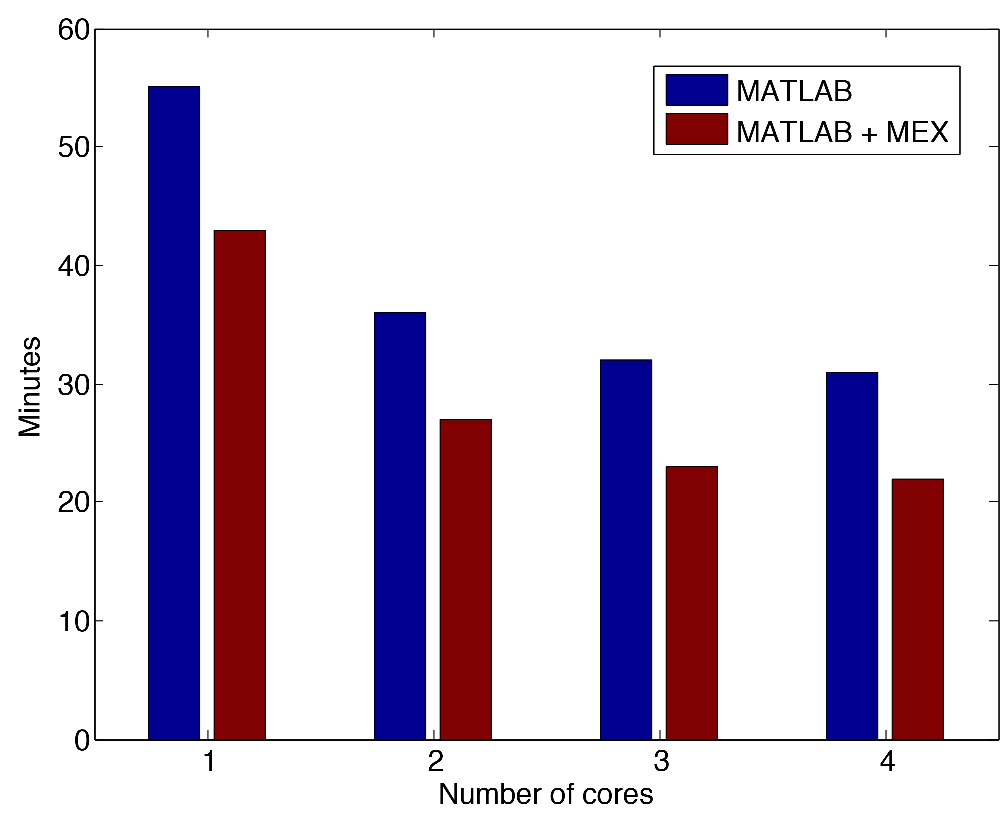
\includegraphics[width=0.5\textwidth]{figures/performance_improvement}
  \caption{Running times of policy training with 2,000 iterations and 150 episodes per iteration, 49 states ($7 \times 7$ grid) and time horizon $T$ equal to the number of states, 49.}
  \label{fig:PerformanceImprovement}
\end{figure}

%!TEX root = thesis.tex

\chapter{Evaluation}
\label{ch:Evaluation}
The implementation of the I-POMDP framework was evaluated by training a policy for the \emph{``Where's Waldo?''} game described in Chapter \ref{ch:IPOMDP} and comparing the performance of the resulting policy to the performance of a greedy policy, a random policy, and a policy that always focuses on the center of the image. 

The policies were trained on a $7 \times 7$ grid where the grid represents the image and each grid location represents a state and an action, i.e. a location where Waldo can be found in and a location the agent can fixate on. The number of actions available to the agent are therefore equal to the number of states, namely $49$.

Both observation models mentioned in Section \ref{sec:ObservationModelImpl} were used to train policies and the default values presented in Section \ref{sec:PolicyTraining} were used in both cases.

\section{Training a Policy Using the Exponential Model}
\label{sec:PolicyExp}
The policy parameters for the policy learned when training with the exponential model for observations can be seen in Figure \ref{fig:ExpPolicyTheta}. This policy favors fixating on locations where the agent's belief is strong, since the values on the diagonal of the policy parameter matrix\footnote{See Section \ref{sec:LogisticPolicies} for an explanation of the policy parameter matrix} are relatively large. An agent using this policy would therefore with a high probability fixate on locations where it beliefs the target is located -- in other words, act greedy.

On both sides of the diagonal we again notice large parameter values, but not as large as on the diagonal itself. This can be interpreted as the second best choice of fixation. Fixating on locations close to the location where the belief is highest will therefore occur with a high probability. This policy could therefore be interpreted as a greedy policy with a slight tendency for curiosity.

\begin{figure}[!htp]
  \centering
  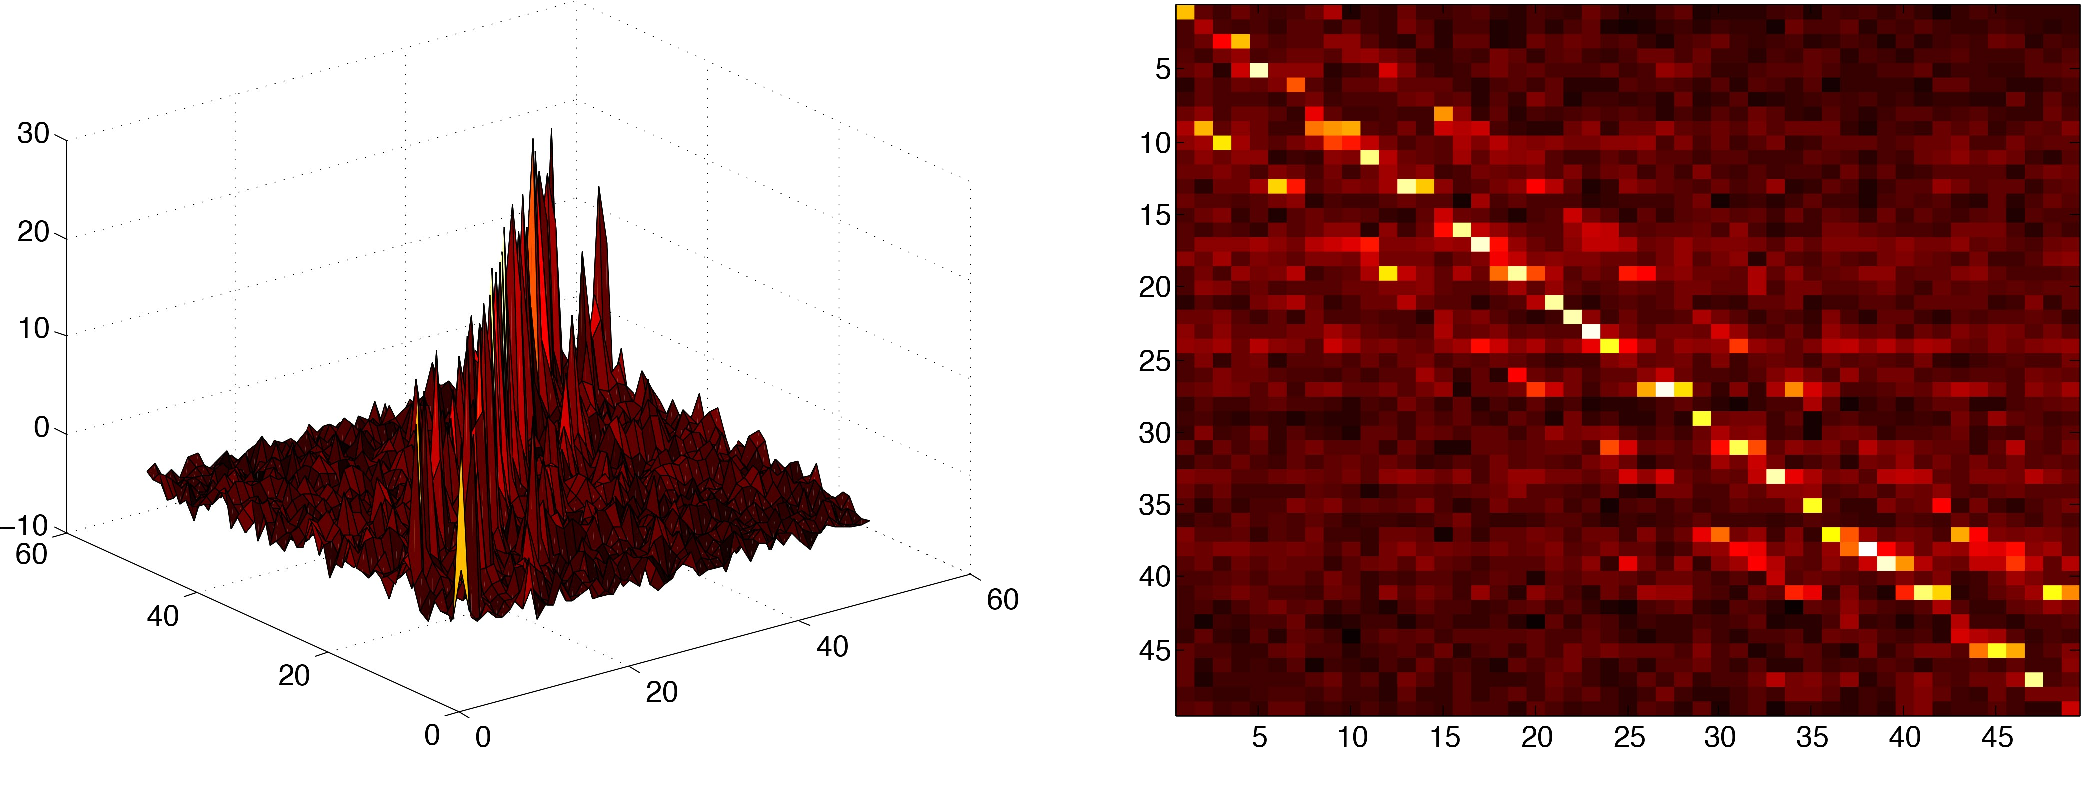
\includegraphics[width=1\textwidth]{figures/exp_policy_theta}
  \caption{The $49 \times 49$ policy parameter matrix $\theta$ trained using the exponential model for observations. \textbf{Left:} Relatively large values on the diagonal, slightly lower values on both sides of the diagonal. \textbf{Right:} The heat map shows clearly the two off-diagonal lines and the relatively large diagonal values.}
  \label{fig:ExpPolicyTheta}
\end{figure}
\FloatBarrier

\noindent
The learning curve for the policy can be seen in Figure \ref{fig:AverageRewardsExp}. It shows that the policy improves fast the first 200 training iterations, as the average rewards in each training iteration get higher and higher (less negative). The policy improvement continues slowly until after around 800 iterations where the learning converges.

\begin{figure}[!htp]
  \centering
  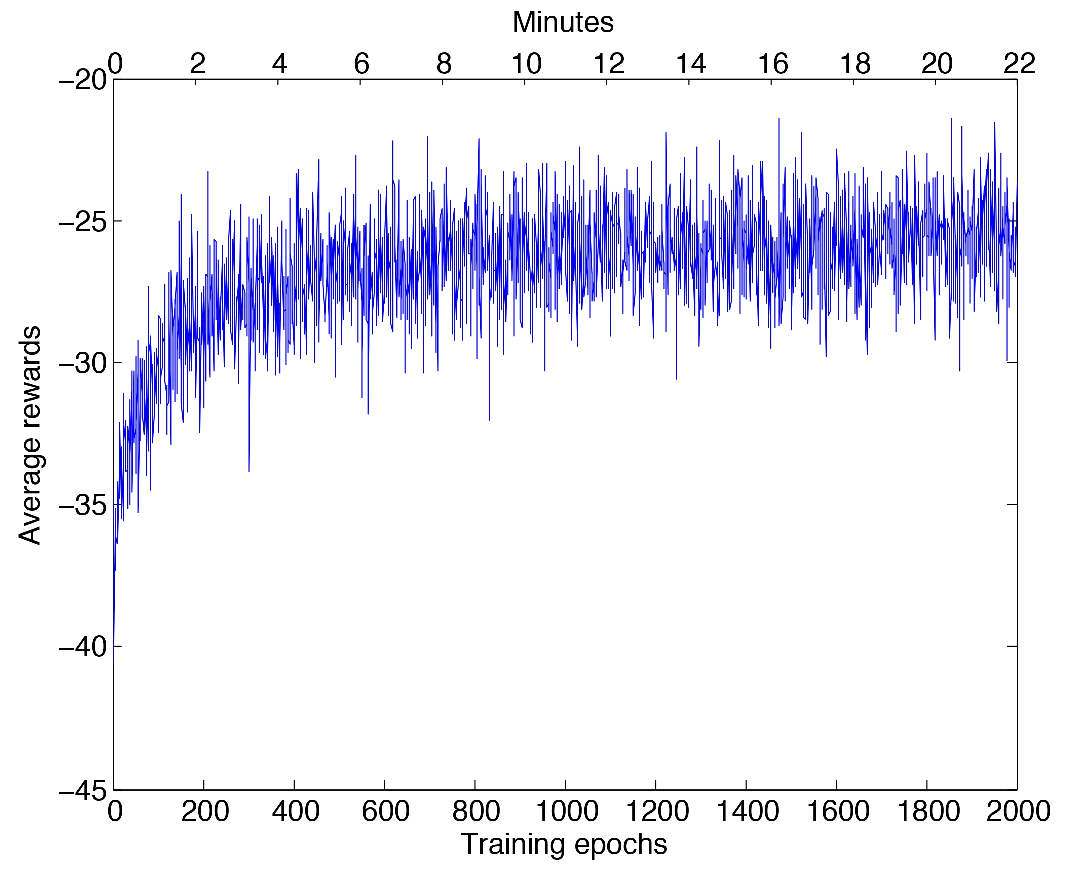
\includegraphics[width=0.5\textwidth]{figures/average_rewards_exp_2x}
  \caption{Average rewards per training iteration while training a policy using the exponential model for observations.}
  \label{fig:AverageRewardsExp}
\end{figure}

\section{Training a Policy Using the Human Eye Model}
The policy parameters for the policy learned when training with the human eye model for observations are very different from the parameters learned in Section \ref{sec:PolicyExp}. Instead of relatively large values on the diagonal, this policy's parameter matrix has less variance in the parameter values but a clear horizontal band of higher values across the middle of it. See Figure \ref{fig:EyePolicyTheta}.

\begin{figure}[!htp]
  \centering
  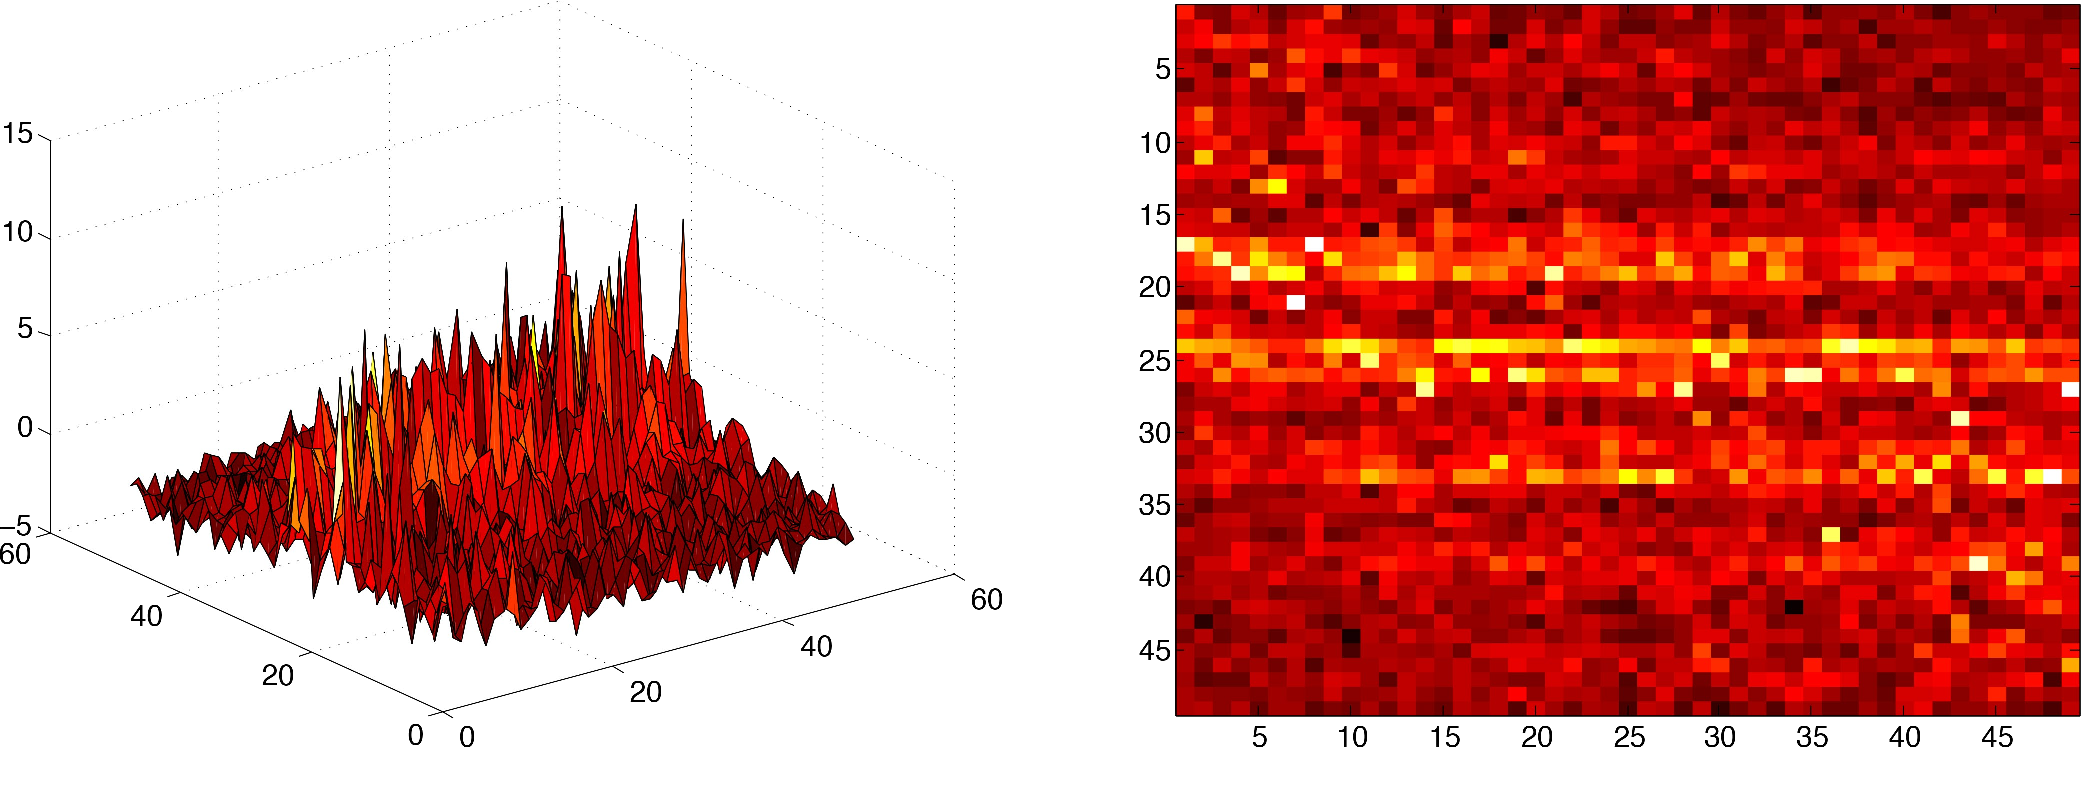
\includegraphics[width=1\textwidth]{figures/eye_policy_theta}
  \caption{The $49 \times 49$ policy parameter matrix $\theta$ trained using the human eye model for observations. \textbf{Left:} Relatively large values across the middle part of the parameter matrix and low values near the top and bottom. \textbf{Right:} Difference between the smallest and largest values not as evident as for the exponential model. Larger values across the center of the matrix.}
  \label{fig:EyePolicyTheta}
\end{figure}
\FloatBarrier

\noindent
To interpret this policy's parameter matrix we first note that on a $7 \times 7$ grid, location number $25$ would be in the center of the grid. With that in mind we can assume that this policy favors fixating on locations around the center of the image.

\begin{figure}[!htp]
  \centering
  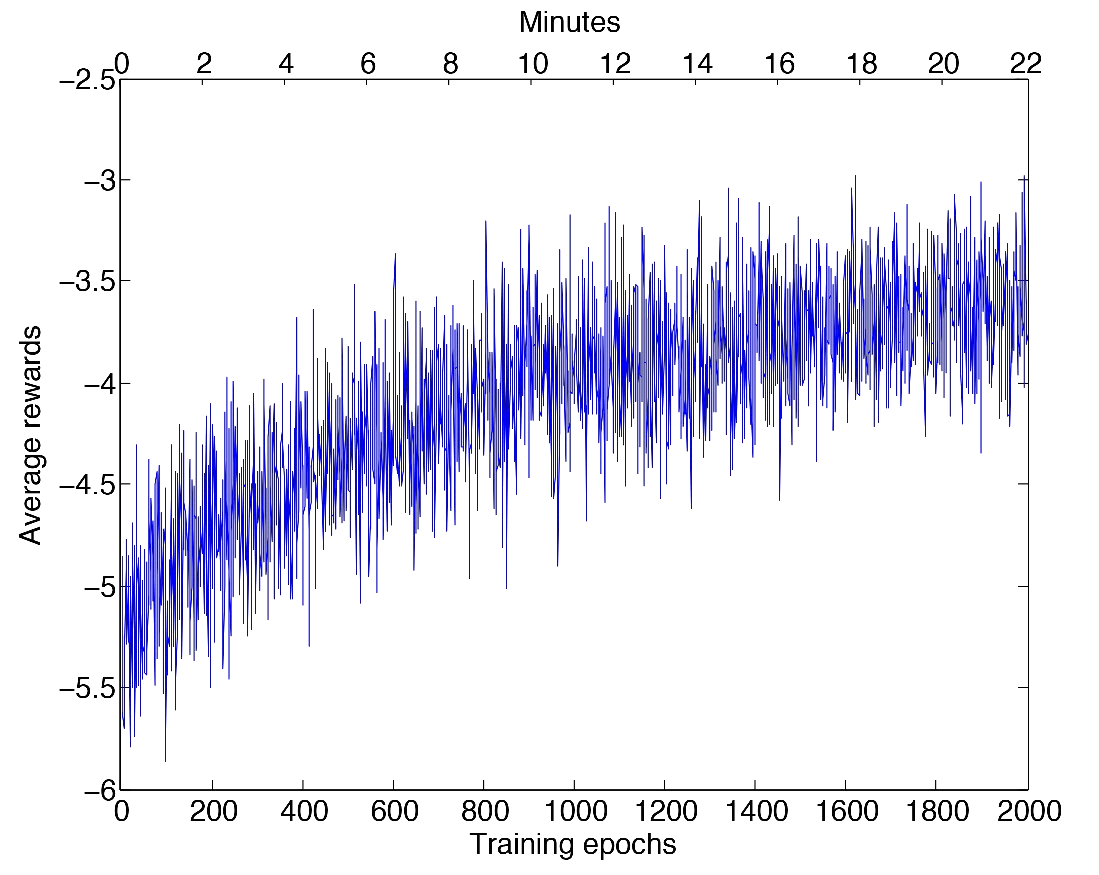
\includegraphics[width=0.5\textwidth]{figures/average_rewards_eye_2x}
  \caption{Average rewards per training iteration while training a policy using the human eye model for observations.}
  \label{fig:AverageRewardsEye}
\end{figure}

\noindent
The learning curve for the policy can be seen in Figure \ref{fig:AverageRewardsEye}. The first thing we notice is that the average rewards per training iteration are higher than during training of the policy in \ref{sec:PolicyExp}. This comes from the fact that the human eye model for observations has a wider field of view than the exponential model, which only sees a small part of the image very clearly.

The policy improves steadily for around 1600 iterations and after that the learning converges.

\section{Performance Comparison}
The performance of both learned policies was compared to the performance of a greedy policy, a random policy, and a policy that always focuses on the center of the image. The comparison was performed by simulating the search for ``Waldo'' with each policy $4,900$ times and recording each time how many fixations it took before the agent's highest belief matched the true location of ``Waldo''.

\subsection{Policy Using an Exponential Model}
All the policies perform similarly for the first 5 fixations, with the trained policy performing slightly better than the others, but after 6 fixations the random policy performs best. The exponential model for observations has a very narrow view and therefore does not fully exploit the potential of the I-POMDP algorithm. For each fixation the agent can only obtain reliable information about the image from the exact location it is fixating on, while the information in the surrounding locations is very noisy. This can make the agent's belief unreliable. As mentioned in Section \ref{sec:PolicyExp} this policy is very similar to the greedy policy and using a greedy policy when the belief is unreliable will result in poor performance. The trained policy is however a stochastic policy and therefore performs better than the greedy policy. The random policy benefits from the fact that it is not dependent on the noisy belief. It should also be noted that a policy that does not fixate on every location will eventually perform worse than random.

The comparison of the policies using the exponential model for observations can be seen in Figure \ref{fig:PolicyComparisonExp}.

\begin{figure}[!htp]
  \centering
  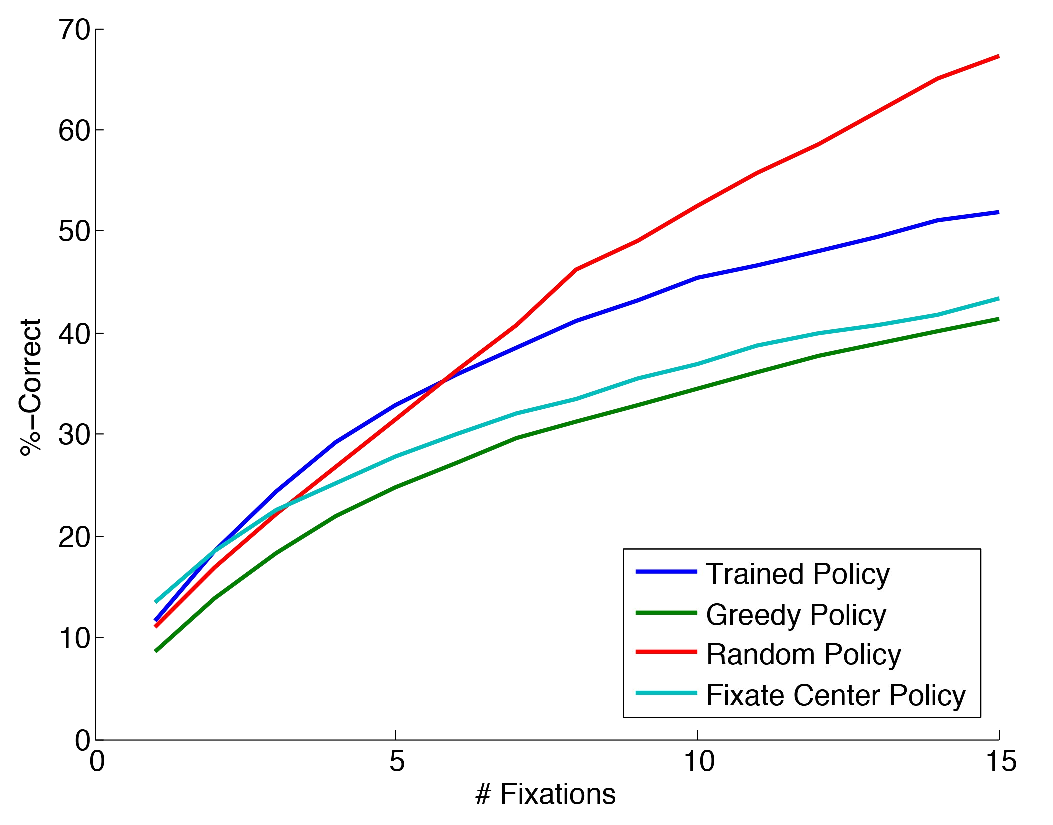
\includegraphics[width=0.5\textwidth]{figures/policy_comparison_exp2}
  \caption{Performance comparison of policies using the exponential model for observations.}
  \label{fig:PolicyComparisonExp}
\end{figure}

\subsection{Policy Using a Human Eye Model}
The human eye model for observations has a wider view than the exponential model and therefore the agent can not only obtain reliable information about the image from the location it fixates on, but also the locations surrounding it. This gives the trained policy an advantage because it exploits the potential of the I-POMDP algorithm. For this reason the trained policy outperforms the other policies as can be seen in Figure \ref{fig:PolicyComparisonEye}.

\begin{figure}[!htp]
  \centering
  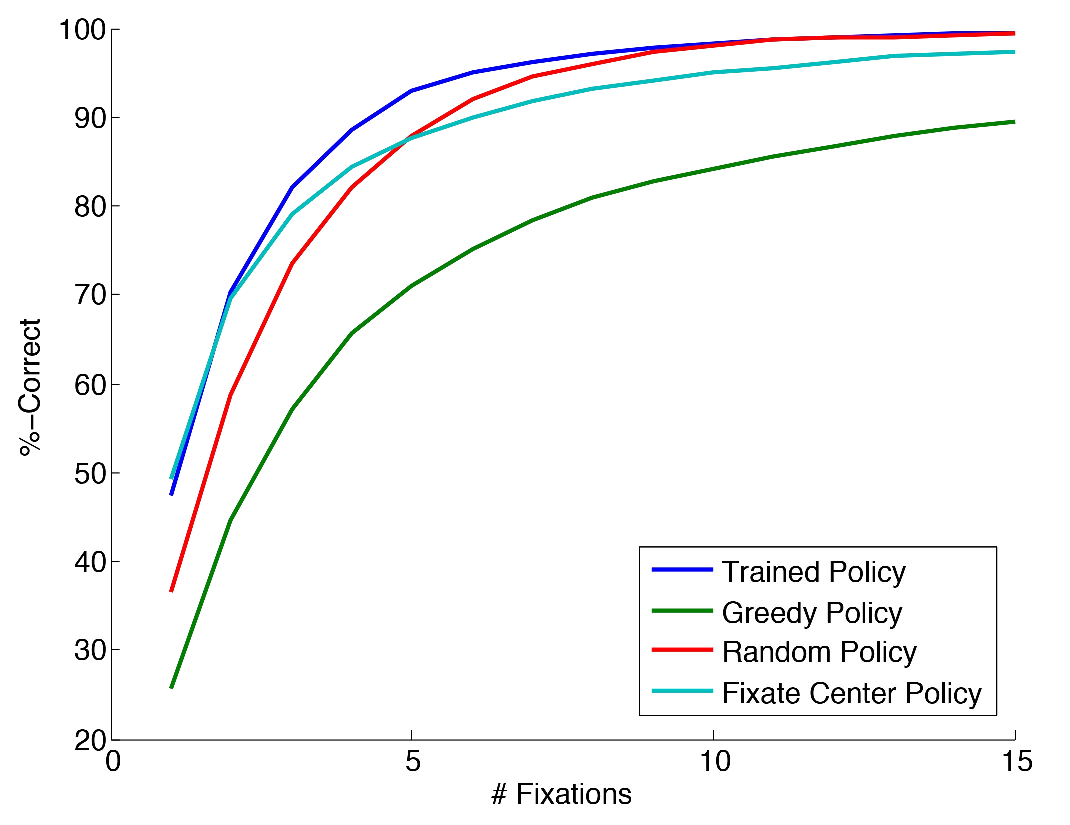
\includegraphics[width=0.5\textwidth]{figures/policy_comparison_eye2}
  \caption{Performance comparison of policies using the human eye model for observations.}
  \label{fig:PolicyComparisonEye}
\end{figure}

\noindent
The greedy policy proves to be a poor strategy in this case as well.

%!TEX root = thesis.tex

\chapter{Conclusions}
\label{ch:Conclusions}
Being able to train a policy that performs well using only intrinsic information is a fascinating idea. It enables us to train policies for agents with no specific tasks other than gathering information. Policies like that can be useful in situations where agents are waiting for tasks and need to be prepared before starting them. They can also be useful for robots that need to interact with humans, since actively gathering information can be important for the robot to be able to resolve human statements. When faced with limitations of sensors and resources such as the field of view of a camera, the range of a microphone or energy for moving around, planning of active information gathering becomes crucial.

In this report we have seen that it is possible to use the I-POMDP framework to train policies that outperform other policies by taking actions that maximize information, but we have also found that the performance of these trained policies depends heavily on the underlying observation model.

Before being able to use the I-POMDP framework to train policies for faster detection of objects in images, a suitable observation model must be constructed. If a suitable model is available, plugging it into the framework is an easy task.

\section{Future Work}
Training policies using the policy gradient method, as it was implemented for this report, required all policy parameters to be updated individually. Since the policy parameters depend on the size of the state- and action spaces, the larger the problem the more challenge it is to train a policy. For object detection in images it is possible to take advantage of shift- and rotation-invariance and tie related parameter values together \cite{Butko2010b}. This can reduce the number of parameters needed to train dramatically.

Another area where the method could be used is in robot exploration. Assume we have a robot with many different sensors for gathering semantic information about its environment. In order for it to gather relative information efficiently it would need to be able to reason about what questions to ask, i.e. which sensor to use, and where and when to ask them. In a scenario like that it would be desirable to learn a policy that chooses questions based on the potential amount of information the answers could provide.


% ------------------------ REFERENCES --------------------------- %
\renewcommand{\bibname}{References}

\bibliographystyle{ieeetr}
\bibliography{references}

% ------------------------- APPENDIX ---------------------------- %
\appendix
\addappheadtotoc
%!TEX root = thesis.tex

\chapter{Derivations and Equations}
\label{app:Derivations}
% --------------------------------------------------------- %
\section{Belief Update}
\label{app:BeliefUpdates}
% --------------------------------------------------------- %
\begin{equation}
  B_t^i \defeq p(S_t = i | A_{1:t}, O_{1:t})
\end{equation}

\begin{subequations}\label{belief_update}
  \begin{align}
    b_t^j &= p(S_t = j | a_{1:t}, o_{1:t})\label{belief_state} \\
          &= \frac{ p(S_t = j, o_t | a_{1:t}, o_{1:t-1}) } { p(o_t) } \\
          &= \frac{ p(o_t | S_t = j, a_{1:t}, o_{1:t-1}) p(S_t = j | a_{1:t}, o_{1:t-1})} { p(o_t) } \\
          \intertext{and since $o_t$ is independent of $o_{1:t-1}$ we can write}
          &= \frac{ p(o_t | S_t = j, a_{1:t}) p(S_t = j | a_{1:t}, o_{1:t-1})} { p(o_t) } \\
          &= \frac{ p(o_t | S_t = j, a_{1:t}) \sum_{i} p(S_t = j, S_{t-1} = i | a_{1:t}, o_{1:t-1})} { p(o_t) } \\
          &= \frac{ p(o_t | S_t = j, a_{1:t}) \sum_{i} p(S_t = j | S_{t-1} = i, a_{1:t}, o_{1:t-1}) p(S_{t-1} = i | a_{1:t-1}, o_{1:t-1})} { p(o_t) } \\
          \intertext{Markovian assumption; given $S_{t-1}$, $S_t$ is independent of $a_{1:t-1}, o_{1:t-1}$ so we get}
          &= \frac{ p(o_t | S_t = j, a_{1:t}) \sum_{i} p(S_t = j | S_{t-1} = i, a_t) p(S_{t-1} = i | a_{1:t-1}, o_{1:t-1}) } { p(o_t) } \\
          \intertext{Using \eqref{belief_state} we can write}
          &= \frac{ p(o_t | S_t = j, a_{1:t}) \sum_{i} p(S_t = j | S_{t-1} = i, a_t) b_{t-1}^i } { p(o_t) } \\
          \intertext{Markovian assumption again; given $S_t$, $o_t$ is independent of $a_{1:t-1}$ so we get}
          &= \frac{ p(o_t | S_t = j, a_t) \sum_{i} p(S_t = j | S_{t-1} = i, a_t) b_{t-1}^i } { p(o_t) }
  \end{align}
\end{subequations}
If the state never changes we have
\begin{equation}\label{fixed_target}
  p(S_t = j | S_{t-1} = i, a_t) =
  \begin{cases}
    1 & \text{if $j = i$} \\
    0 & \text{otherwise}
  \end{cases}
\end{equation}
and then \eqref{belief_update} becomes
\begin{equation}\label{belief_update_fixed}
  b_t^j = \frac{ p(o_t | S_t = j, a_t) b_{t-1}^j }{ p(o_t) }
\end{equation}
where $p(o_t)$ can be treated as a normalization factor.

% --------------------------------------------------------- %
\section{Observations}
% --------------------------------------------------------- %
The observation model is
\begin{equation}\label{app:ObservationModel}
  \begin{split}
    O_t^j &= \delta (S_t, j) d_{j,k} + Z_t^j \\
          &= \begin{cases}
                d_{j,k} + Z_t^j & \text{if $S_t = j$}\\
                Z_t^j           & \text{otherwise}
             \end{cases}
  \end{split}
\end{equation}
where $Z_t^j$ is zero mean, unit variance Gaussian random noise (i.e. white noise) and in the case of an exponential-decay vision system 
\begin{equation}
  d_{j,k} = 3 \cdot e^{-dist(j,k)}
\end{equation}
where $dist(j,k)$ is the Euclidean distance between locations $j$ and $k$.

We assume that given an image, individual observations (i.e. each pixel)
\begin{equation}
  o_t = (o_t^1, \dotsc, o_t^{|\mathcal{S}|})
\end{equation}
are conditionally independent. Then we can write the probability of an observation as
\begin{subequations}
  \begin{align}
    p(o_t | S_t = i, A_t = k) 
      &= \prod_j p(o_t^j | S_t = i, A_t = k) \\
      &= p(o_t^i | S_t = i, A_t = k) \prod_{j \neq i} p(o_t^j | S_t = i, A_t = k) \\
      \intertext{Given the observation model from equation \eqref{app:ObservationModel} we get}
      &= \gaussianexp{o_t^i - d_{i,k}} \prod_{j \neq i} \gaussianexp{o_t^j} \\
      &= \frac{1}{\sqrt{2\pi}} \frac{\gaussianexppart{o_t^i - d_{i,k}}}{\gaussianexppart{o_t^i}} \prod_j \gaussianexp{o_t^j} \\
      &= \frac{\gaussianexppart{o_t^i - d_{i,k}}}{\gaussianexppart{o_t^i}} Z \\
      &= \exp((o_t^i - \frac{d_{i,k}}{2}) d_{i,k}) K
  \end{align}
\end{subequations}
where $K$ is a constant. Ignoring the constant $K$ and terms not containing $o_t^i$ we can write
\begin{equation}
  \label{app:ProportionalObservationLikelihood}
  p(o_t | S_t = i, A_t = k) \propto \exp{(d_{i,k} o_t^i)}
\end{equation}

% --------------------------------------------------------- %
\section{Proportional Belief Update}
% --------------------------------------------------------- %
Combining \eqref{belief_update_fixed} and \eqref{app:ProportionalObservationLikelihood} yields the proportional belief update
\begin{equation}
  % b_{t+1}^i \propto \exp(\alpha_{i,k} d_{i,k}) b_t^i
  b_{t+1}^i \propto \exp{(d_{i,k} o_t^i)} b_t^i
\end{equation}

%!TEX root = thesis.tex

\chapter{MEX Function for Calculating Policy Gradient}
\label{app:GradientCImplementation}
\lstset{language=C++,columns=fullflexible,breaklines=true}
\lstinputlisting{thesis-implementation/get_gradient.cc}


\clearpage
\thispagestyle{empty}
\includepdf[pages={2}, pagecommand={}]{kth-cover.pdf}

\end{document}
